\begin{frame}{Metric Facility Location}
  \begin{block}{Definicja problemu}
    Mamy dane zbiory punktów $F$ - fabryk oraz $C$ - miast. \\
    Funkcja kosztu otwarcia fabryki $o: F \rightarrow \mathbb{R}$. \\
    Funkcja połączenia fabryki z miastem $c: (F \times C) \rightarrow \mathbb{R}$. \\
    $c$ spełnia warunek trójkąta. \\
    Cel: znaleźć taki podzbiór fabryk $F'$ i takie przypisanie $a$ fabryk do miast, aby
    suma $\sum_{f \in F'}o(f) + \sum_{i \in C}c(a(i), i)$ była minimalna.
  \end{block}
\end{frame}

\begin{frame}{Metric Facility Location}
  \begin{block}{Jak trudny jest ten problem?}
    \pause
    Odp: NP - trudny
  \end{block}
\end{frame}

\begin{frame}{Metric Facility Location}
  \begin{block}{Czego próbowaliśmy?}
    \begin{itemize}
      \item Metoda prymalno-dualna (programowanie liniowe) (3 - aproksymacja)
      \item Losowe rozwiązanie. 
      \item Local search (3 - aproksymacja)
      \item MCTS (o tym później)
    \end{itemize}
  \end{block}
\end{frame}

\begin{frame}{Metric Facility Location}
  \begin{block}{Metoda prymalno-dualna}
    \begin{itemize}
      \pause
      \item Definiujemy problem jako zagadnienie programowania liniowego i je aproksymujemy.
      \pause
      \item Nam służy tylko jako referencja do naszych wyników.
      \pause
      \item Jain i Vasirani
    \end{itemize}
  \end{block}

  \pause

  \begin{block}{Losowe rozwiązanie}
    \begin{itemize}
      \item Zwykle jednostajne losowanie.
      \item Tylko referencja.
    \end{itemize}
  \end{block}
\end{frame}


\begin{frame}{Metric Facility Location}
  \begin{block}{Local search}
    \begin{itemize}
      \pause
      \item Przestrzeń rozwiązań - wszystkie podzbiory $F$. (dużo)
      \pause
      \item Poprawne ruchy:
        \begin{itemize}
          \item dołączamy fabrykę do zbioru otwartych fabryk
          \item usuwamy fabrykę ze zbioru otwartych fabryk
          \item usuwamy i dodajemy jedną fabrykę
        \end{itemize}
    \end{itemize}
  \end{block}

  \pause
  \begin{block}{Local search - jak wybieramy poprawny ruch?}
    Dwie strategie:
    \begin{itemize}
      \item Losowo - $O(|F|\cdot |C|)$
      \item Najbardziej poprawiający wynik - $O(|F|(|F| + |C|))$
    \end{itemize}
  \end{block}
\end{frame}

\begin{frame}
\pgfsetplotmarksize{0pt}
\begin{figure}
 \centering
 \caption{\label{fl_conv0}FLClustered/test0.txt},
 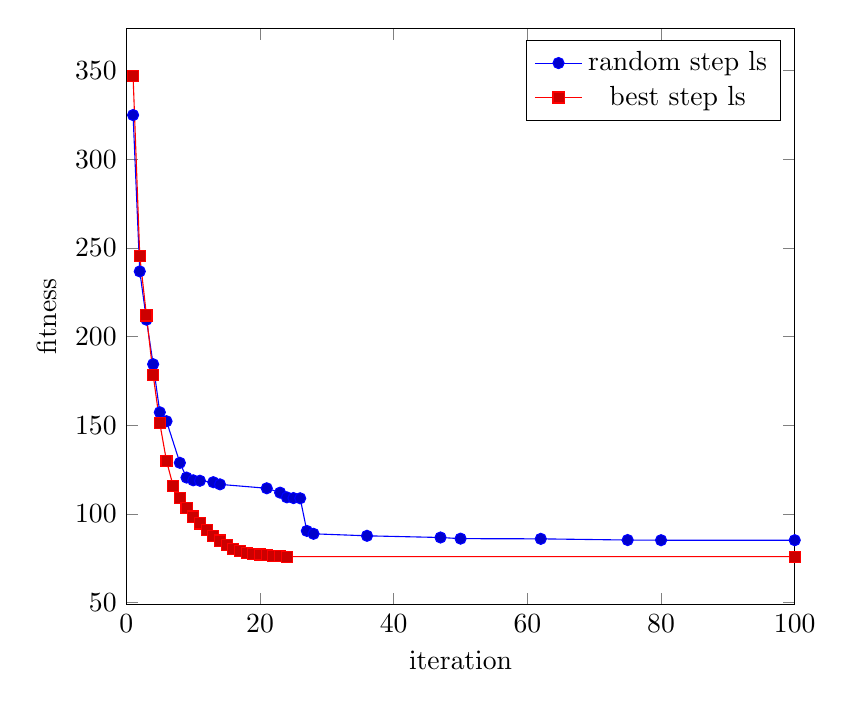
\begin{tikzpicture}
 \begin{axis}[
   width=0.7\textwidth,
   scale only axis,
   xlabel=iteration,
   ylabel=fitness,
   xmin=0,xmax=100,
   domain=0:100]
   \addplot coordinates {
     (0,inf)
     (1,324.942)
     (2,236.782)
     (3,209.541)
     (4,184.435)
     (5,157.321)
     (6,152.289)
     (8,128.823)
     (9,120.497)
     (10,118.965)
     (11,118.708)
     (13,117.899)
     (14,116.674)
     (21,114.465)
     (23,112.007)
     (24,109.374)
     (25,108.944)
     (26,108.819)
     (27,90.4234)
     (28,88.7929)
     (36,87.6585)
     (47,86.7098)
     (50,86.0617)
     (62,85.9504)
     (75,85.279)
     (80,85.1812)
     (100,85.1812)
   };
   \addlegendentry{random step ls}
   \addplot coordinates {
     (0,inf)
     (1,346.828)
     (2,245.422)
     (3,211.931)
     (4,178.561)
     (5,151.073)
     (6,129.859)
     (7,115.752)
     (8,108.788)
     (9,103.321)
     (10,98.5095)
     (11,94.646)
     (12,90.7951)
     (13,87.4437)
     (14,84.9935)
     (15,82.5473)
     (16,80.3739)
     (17,78.9966)
     (18,78.1543)
     (19,77.4955)
     (20,77.1273)
     (21,76.7786)
     (22,76.46)
     (23,76.0552)
     (24,75.926)
     (100,75.926)
   };
   \addlegendentry{best step ls}
 \end{axis}
 \end{tikzpicture}
\end{figure}

\end{frame}

\begin{frame}
\pgfsetplotmarksize{0pt}
\begin{figure}
 \centering
 \caption{\label{fl_conv6}UflLib/Euclid/1011EuclS.txt},
 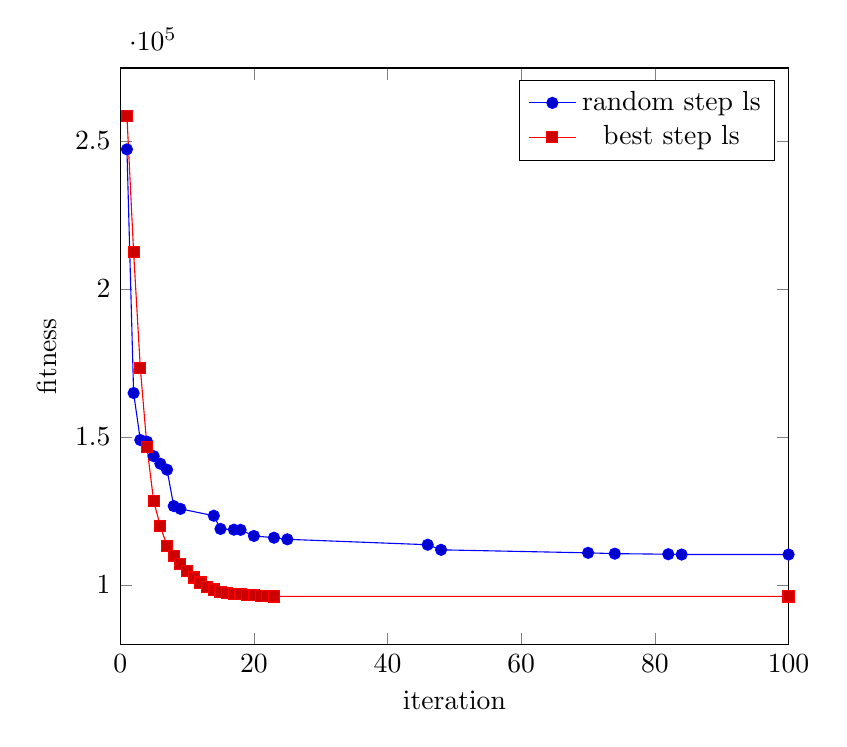
\begin{tikzpicture}
 \begin{axis}[
   width=0.7\textwidth,
   scale only axis,
   xlabel=iteration,
   ylabel=fitness,
   xmin=0,xmax=100,
   domain=0:100]
   \addplot coordinates {
     (0,inf)
     (1,247173)
     (2,164855)
     (3,148983)
     (4,148438)
     (5,143524)
     (6,140956)
     (7,138947)
     (8,126665)
     (9,125722)
     (14,123396)
     (15,118937)
     (17,118697)
     (18,118633)
     (20,116575)
     (23,115980)
     (25,115436)
     (46,113604)
     (48,111881)
     (70,110862)
     (74,110592)
     (82,110399)
     (84,110288)
     (100,110288)
   };
   \addlegendentry{random step ls}
   \addplot coordinates {
     (0,inf)
     (1,258418)
     (2,212384)
     (3,173393)
     (4,146526)
     (5,128358)
     (6,119830)
     (7,113211)
     (8,109737)
     (9,107133)
     (10,104709)
     (11,102534)
     (12,100826)
     (13,99429)
     (14,98453)
     (15,97721)
     (16,97269)
     (17,96972)
     (18,96841)
     (19,96724)
     (20,96670)
     (21,96416)
     (22,96355)
     (23,96135)
     (100,96135)
   };
   \addlegendentry{best step ls}
 \end{axis}
 \end{tikzpicture}
\end{figure}

\end{frame}
